
\chapter{Primitive Data Types}

\section{Boolean}
\iffalse
https://oopscenities.net/2011/09/28/c-primitive-types/
https://en.wikipedia.org/wiki/Primitive_data_type
http://rypress.com/tutorials/objective-c/data-types/primitives
https://en.wikipedia.org/wiki/C_data_types
\fi
\section{Character}

\section{Floating-point}

\section{Integer}

\section{Enumeration}


\chapter{Composite Data Types}
\section{Record - struct or class}
\section{Union}
\section{Tagged Union}


\chapter{Array}
Array belongs to the so called \textit{Contiguous} Data Structure in which stored elements (all of the same type) are arranged in a \textbf{single} slab of memory. Array's elements can be easily  accessed given their \textit{indices} within the array itself the same way, using an analogy, we can locate an house in a specific street given its postcode. Array can also be tought as a collection of variables of the same type.

Major characteristic of arrays are:
\begin{description}
\item [Constant time access] All the element of the array can be accessed in $\mathcal{O}(1)$. Array can be fully described by its
	\begin{enumerate}
		\item Starting address $m_0$
		\item Size of Stored data type (e.g. 4 bytes for \texttt{int} or 1 byte for \texttt{char}) $S$
		\item Number of stored elements (i.e. array length) $L$
	\end{enumerate}
	\begin{figure}[h]
		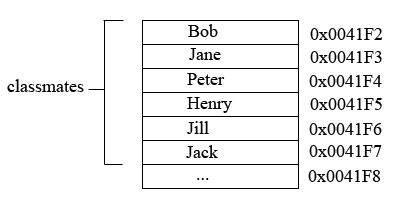
\includegraphics[width=8cm]{array1.png}
	\end{figure}
	The starting address correnspond to the first element (in C-like languages index $0$) element.
	 The second element starts at the address  $m_0 + S$, third at $m_0 + S + S$ and so on. so the element at index $i$ has index $s_i = m_0 +iS$.
	
\item [Only Data] Array are space efficient because they do not store any other information but data itself (unlike list for instance where each node of the list stores a pointer to the next element of the list). 
 
\item [Memory locality] Array adhere perfectly to the principle of spatial locality\footnote{If a particular memory location is referenced at a particular time, then it is likely that nearby memory locations will be referenced in the near future. In this case it is common to attempt to guess the size and shape of the area around the current reference for which it is worthwhile to prepare faster access.} in which related storage locations are frequently accessed (iterating through an array is a very common idiom in all programming languages). This allows cache to work at his best.
\end{description}

Arrays have fixed size, and this in several application is a major downside (the size of the array is input dependent for instance). C-like languages allow for dynamic memory allocation at runtime (see \ref{chap:malloc} at page (\pageref{{chap;malloc}}). This involves the creation of a (different) larger (how larger is an important point) array and the copy of the first one in the beginning of the newly created one. If the program requires this dynamic enlarging often we could end up wasting much time in copying data here and there.
The common strategy used for creating a dynamic array is to double the size of the array each time. This mitigate the average number of copies of each element. Let's imagine we start with an array of size one and we try to insert $n$ elements, doubling the size of the array when its capacity its full. The first element is has to be copied when the array expands after the fist, second, fourth, eighth ... $2^i = n$ insertion.
It will take $i = log(n)$ doubling size for the array to have size $n$. Element in the last half of the array will be copied only one (at the last doubling). A quarter of the elements will be copied twic and so on. The total number of copies will be then
\[
M = \sum_{i=1}^{\log(n)} \frac{ni}{2^i} = n\sum_{i=1}^{\log(n)} \frac{i}{2^i} = n(\frac{1}{2}+\frac{1}{2} + \frac{3}{8} + \frac{1}{3} ... \frac{log(n)}{n})=2n
\]
So in average  each element is copied only two times.

 \section{Problems and Solution}

%---Problem---------------------------------
\begin{problem}
Given an array, $A$, of $N$ integers, print each element in reverse order as a single line of space-separated integers.
\end{problem}	

\begin{solution}

		\begin{lstlisting}[language=C, caption="C"]
        int main(){
    int n; 
    scanf("%d",&n);
    int *arr = malloc(sizeof(int) * n);
    for(int arr_i = 0; arr_i < n; arr_i++){
       scanf("%d",&arr[arr_i]);
    }
    while(--n >=0){
       printf("%i ",arr[n]);
    }
    
    return 0;
}

		\end{lstlisting}  

\end{solution}	
%------------------------------------------------ 
 
  \begin{problem}
	Reverse an array in place.
 \end{problem}
 
 \begin{problem}
    Implement a function to determine if a string has all unique characters. String can only contains latin 	characters. What happen if you are forced to use no additional data structures?
\end{problem}

 \begin{problem}
    Implement a function to determine if a string has all unique characters. String can only contains latin 	characters. What happen if you are forced to use no additional data structures?
\end{problem}

 \begin{problem}
    Implement a function to determine the number of repeated characters in a string. (e.g. google has 2 repeated characters, \textit{g} and \textit{o}).
\end{problem}

 \begin{problem}
   Given an array of integer of given size containing numbers from 1 to $N \geq 2$ . Only one number is missing within the array. Write a function which output is that missing number.
\end{problem}

 \begin{problem}
   Given an array of integer of size $N$ containing numbers from 1 to $N-2$. All numbers appear only once except one which is repeated twice. Write a function which return that number.
\end{problem}

 \begin{problem}
Write a function which find the smallest and largest number in an unsorted array of integers. 
\end{problem}

 \begin{problem}
	Sort an array of integer using a $\mathcal{O}(n^2)$  and a $\mathcal{O}(nlog(n))$  algorithm. Both algorithm should sort the array \textit{in-place}.
\end{problem}

 \begin{problem}
	Given two array of sorted integer, \textit{A,B} find their intersection i.e. an array $C$ which contains only elements which belong both to A and B. $C=\{c_i \;|\; c_i \in A;,\; c_i \in B\}$
\end{problem}

 \begin{problem}
	Given two array of unsorted integer in which only one element is repeted (the rest of them appear only once). Write a function which finds that element in $\mathcal{O}(n)$  time.
\end{problem}

 \begin{problem}
	Write a function which finds the kth largest element in a unsorted array.
\end{problem}
 \begin{problem}
	Write a function which finds the kth smallest element in a unsorted array.
\end{problem}

 \begin{problem}
Count the number of distinct ( (a,b) is not distinct from (b,a) ) pairs in an array of integers which sum is equal to a given value $K$.
\end{problem}

 \begin{problem}
Given three sorted array (in non decreasing order) find the intersection between all of their elements.
\end{problem}

 \begin{problem}
Given an array, find the first repeated element. i.e. an element $e$ which occurs more than once and which index is the smallest. On the following input $1,2,3,4,5,3,2,2,7$ the function should return two because is the a repeated element with the smallest index (1).
\end{problem}

 \begin{problem}
Given an array, return the larger and the 2th-largst element.
\end{problem}


 \begin{problem}
Given an array of integer, find the smallest positive integer which cannot be represented as sum of any subset of the array. On  input 1, 3, 6, 10, 11, 15 the function should return 2. Note that the array can also contains negative numbers.
\end{problem}

 \begin{problem}
Given an array of integer (positive and negative), return an array which elements are rearranged in alternating positive and negative. You are ensured that the number of positives and negatives matches. E.g. on input $(1,2,-6,4,8,-6,-5)$ the functions (only one of the possible valide output) return $(1,-6,2,-6,4,-5,8)$.
\end{problem}

 \begin{problem}
Given an array of integer write a function which return true is a non empty subset of its element which sum up to $0$. False otherwise. 
\end{problem}

 \begin{problem}
Given an array $A$ of integer find the length of the  longest sequence of consecutive integers. On input $1,56,8,-5,3,7,4,23,2,5)$ the function should return 5 (is the length of the consecutive subsequence $(1,2,3,4,5)$)
 \end{problem}

 \begin{problem}
Find the minimum in a rotated sorted array. (a rotation of $1,2,3,4,5,6$ could be for instance $4,5,6,1,2,3$). The array does not contains duplicates.

What if we allows for duplicated to be present? How does this changes the overall time complexity?
 \end{problem}

 \begin{problem}\label{array:anagram}
Given two string, determine which is the minimum number of deletions (a delete operation can be performed on both string) necessary for the two string to be a valid anagram\footnote{A word, phrase, or name formed by rearranging the letters of another, such as spar, formed from rasp.} of each other. Strings contains only latin characters with no space. Given \textit{hello} and \textit{belloz} the function should returns 2. ( See solution \ref{array:anagram_sol} at page \pageref{array:anagram_sol} )


\begin{lstlisting}[ label=array:anagram_sol, caption=Solution to problem \ref{array:anagram} ]
#include <stdio.h>
#include <string.h>
#include <math.h>
#include <stdlib.h>

void removeTrailingNL(char* s){
    int size = strlen(s);
    if(size > 0 && s[size-1] == '\n')
        s[size-1] = '\0';
}

#define MAX_INPUT_SIZE (10000)
int main() {
    const int alph_size = 'z'-'a'+1;
    int s1_freq[alph_size];
    int s2_freq[alph_size];
    //initialize frequencies arrays
    for(int i = 0 ; i < alph_size ; i++){
        s1_freq[i] = 0;
        s2_freq[i] = 0;
    }
    //read both string
    char s1[10000];
    char s2[10000];
    fgets(s1,MAX_INPUT_SIZE,stdin);
    fgets(s2,MAX_INPUT_SIZE,stdin);
    removeTrailingNL(s1);
    removeTrailingNL(s2);
    
    int size_s1, size_s2;
    size_s1 = strlen(s1);
    size_s2 = strlen(s2);
    //compute frequencies
    for(int i  = 0 ; i< size_s1 ; i++)
        s1_freq[s1[i]-'a'] = s1_freq[s1[i]-'a'] + 1;
    for(int i  = 0 ; i< size_s2 ; i++)
        s2_freq[s2[i]-'a'] = s2_freq[s2[i]-'a'] + 1;
    /*
  //print frequencies  
 for(int i  = 0 ; i< alph_size ; i++){
     printf("%c %i %i\n",'a'+i,s1_freq[i],s2_freq[i]);
 }*/
    
    //compute minimum delete operation
    int dels = 0;
    for(int i  = 0 ; i< alph_size ; i++)
        dels = dels + (abs(s1_freq[i] - s2_freq[i]));
    
    
    //prints output
    printf("%i",dels);
   
    return 0;
}
\end{lstlisting}
 \end{problem}






\chapter{List}
\section{Singly Linked List}
\section{Doubly Linked List}
\section{Circular Linked List}
\section{Self-Organizing Lists}
\section{Skip Lists}

\chapter{Stack}

\chapter{Queue}
\section{Double-ended queue - Dequeue}

\section{Priority Queue}
Nevertheless, the heap data structure itself has enormous utility. In this section, we present one of the most popular applications of a heap: its use as an efficient priority queue.
A priority queue is a data structure for maintaining a set S of elements, each with an associated value called a key. A priority queue supports the following operations.
\begin{description}
\item [\texttt{INSERT(S,x)}] inserts an element $x$ into the set S
\item [\texttt{\{MAX,MIN\}(S,x)}] return the element of S with largest/smallest key 
\item [\texttt{EXTRACT-\{MAX,MIN\}(S,x)}] return and removes the element of S with largest/smallest key 
\end{description}
One application of priority queues is to schedule jobs on a shared computer. The priority queue keeps track of the jobs to be performed and their relative priorities. When a job is finished or interrupted, the highest-priority job is selected from those pending using EXTRACT-MAX. A new job can be added to the queue at any time using INSERT.

A priority queue can also be used in an event-driven simulator. The items in the queue are events to be simulated, each with an associated time of occurrence that serves as its key. The events must be simulated in order of their time of occurrence, because the simulation of an event can cause other events to be simulated in the future. For this application, it is natural to reverse the linear order of the priority queue and support the operations MINIMUM and EXTRACT-MIN instead of MAXIMUM and EXTRACT-MAX. The simulation program uses EXTRACT-MIN at each step to choose the next event to simulate. As new events are produced, they are inserted into the priority queue using INSERT.

Not surprisingly, we can use a heap to implement a priority queue. The operation HEAP-MAXIMUM returns the maximum heap element in (1) time by simply returning the value A[1] in the heap. The HEAP-EXTRACT-MAX procedure is similar to the for loop body (lines 3-5) of the HEAPSORT procedure:

\begin{algorithm}[H]
 \KwData{Heap H}
 \KwResult{Extract Max - Max element of H}
\uIf{heap-size(H) $<$ 1}{
	 underflow error
   }

$max \gets H[1]$\;
$H[1] \gets H[heap-size(H)]$\;
$heap-size(H) \gets heap-size(H) -1$\;
\Return{max}\;

\caption{Priority Queue Extract-max pseudocode}
\end{algorithm}

The running time of HEAP-EXTRACT-MAX is $\mathcal{O}(log n)$, since it performs only a constant amount of work on top of the $\mathcal{O}(log n)$ time for HEAPIFY.

The HEAP-INSERT procedure inserts a node into heap A. To do so, it first expands the heap by adding a new leaf to the tree. Then, in a manner reminiscent of the insertion loop of INSERTION-SORT (see section \ref{sec:insertionsort} at page \pageref{sec:insertionsort}), it traverses a path from this leaf toward the root to find a proper place for the new element.

\begin{algorithm}[H]
 \KwData{Heap H, Key key}
 \KwResult{Insert an element in the Heap H}
	$heap-size(H) \gets heap-size(H)+1$\;
	$i \gets heap-size(H)$\;
	\While{$i > 1 and H[parent(i)] < key$}{
		$H[i] \gets H[parent(i)]$\;
		$i \gets parent(i)$\;
	}
	$H[i] \gets key$
\caption{Priority Queue insert pseudocode}
\end{algorithm}

\begin{problem}
Show how to implement a first-in, first-out queue with a priority queue. Show how to implement a stack with a priority queue.
\end{problem}


\begin{problem}

Give an O(lg n)-time implementation of the procedure HEAP-INCREASE-KEY(A, i, k), which sets A[i]  max(A[i],k) and updates the heap structure appropriately.
\end{problem}

\begin{problem}

The operation HEAP-DELETE(A, i) deletes the item in node i from heap A. Give an implementation of HEAP-DELETE that runs in O(lg n) time for an n-element heap.
\end{problem}

\begin{problem}

Give an O(n lg k)-time algorithm to merge k sorted lists into one sorted list, where n is the total number of elements in all the input lists. (Hint: Use a heap for k-way merging.)
\end{problem}


\begin{problem}

A d-ary heap is like a binary heap, but instead of 2 children, nodes have d children.
\begin{enumerate}
\item How would you represent a d-ary heap in an array?
\item What is the height of a d-ary heap of n elements in terms of n and d?
\item Give an efficient implementation of EXTRACT-MAX. Analyze its running time in terms of d and n.
\item Give an efficient implementation of INSERT. Analyze its running time in terms of d and n.
\item Give an efficient implementation of HEAP-INCREASE-KEY(A, i, k), which sets A[i]  max(A[i], k) and updates the heap structure appropriately. Analyze its running time in terms of d and n.
\end{enumerate}
\end{problem}








\chapter{Heap}


\chapter{Tree}

\section{Binary Tree}
\section{Binary Search Tree}

\section{Self Balancing Tree}
\subsection{B Tree}
\subsection{B+ Tree}

\subsection{Adelson-Velsky Landis Tree - AVL Tree}
\subsection{Red Black Tree}
\subsection{Splay Tree}


\section{Space-partitioning trees}
\subsection{Kd Tree}
\subsection{R Tree}

%-----CHAPTER GRAPH---------------------------
\chapter{Graph}


\section{Exercices}

%---Problem------------
\begin{problem}
The incidence matrix of a directed graph $G=(V,E)$ with s.t. $E$ is a not reflexive relation  is a
$V \times E$ matrix $B = b_{ij}$ such that:
\[
    b_{ij}=\left\{
                \begin{array}{ll}
                  -1 &\text{if j leaves i}\\
                  1 &\text{if j enters i}\\
                  0 &\text{otherwise}
                \end{array}
              \right.
  \]
What the entries of $BB^T$ represents?

	\begin{solution}
	
	\end{solution}
\end{problem}





%---Problem------------
\begin{problem}
\textit{Given an adjacency-list representation of a directed graph, how long does it take
to compute the out-degree of every vertex? How long does it take to compute the
in-degrees?}

	\begin{solution}
\begin{itemize}
\item Out-degree is easy since each node stores the adjacency information as out edges. So out-degree is simply the length of the list which is usually stored as list's attribute hence accessible in $O(1)$. If it 
is the case the time complexity is $O(|V|)$ otherwise we need to inspect all the edges yelding to a $O(|E|)$. 
\item In-degree for node $i$ requires to collect adjacency information from all the other nodes $j \neq i$. Complexity is $O(|E|)$.
\end{itemize}

	\end{solution}
\end{problem}




%---Problem------------
\begin{problem}
\textit{Give an adjacency-list representation for a complete binary tree on 7 vertices. Give
an equivalent adjacency-matrix representation. Assume that vertices are numbered
from 1 to 7 as in a binary heap.}

\begin{solution}

\begin{description}

\item [Adjancency Matrix]\hfill \\
\begin{tabular}{|l|l|l|l|l|l|l|l|}
\hline
\textbf{}  & \textbf{1} & \textbf{2} & \textbf{3} & \textbf{4} & \textbf{5} & \textbf{6} & 7          \\ \hline
\textbf{1} & \textit{0} & \textit{1} & \textit{1} & \textit{0} & \textit{0} & \textit{0} & \textit{0} \\ \hline
\textbf{2} & \textit{0} & \textit{0} & \textit{0} & \textit{1} & \textit{1} & \textit{0} & \textit{0} \\ \hline
\textbf{3} & \textit{0} & \textit{0} & \textit{0} & \textit{0} & \textit{0} & \textit{1} & \textit{1} \\ \hline
\textbf{4} & \textit{0} & \textit{0} & \textit{0} & \textit{0} & \textit{0} & \textit{0} & \textit{0} \\ \hline
\textbf{5} & \textit{0} & \textit{0} & \textit{0} & \textit{0} & \textit{0} & \textit{0} & \textit{0} \\ \hline
\textbf{6} & \textit{0} & \textit{0} & \textit{0} & \textit{0} & \textit{0} & \textit{0} & \textit{0} \\ \hline
\textbf{7} & \textit{0} & \textit{0} & \textit{0} & \textit{0} & \textit{0} & \textit{0} & \textit{0} \\ \hline
\end{tabular}
\hfill \\
\item [Adjancency list] \hfill \\
\begin{verbatim}
1:  2 -> 3 -> NIL
2:  3 -> 4 -> NIL
3:  5 -> 6 -> NIL
4: NIL
5: NIL
6: NIL
7: NIL
\end{verbatim}
\end{description}
\end{solution}
\end{problem}

%---Problem------------
\begin{problem}
The transpose of a directed graph $G = (V,E)$  is the graph $G = (V,E^T)$, where
$ E^T = \{ (v,u) \in V \times V \: : \: (u,v) \in E \}$. Thus $G^T$ is $G$ with all edges reversed.
Describe an efficient algorithm for computing $G^T$ for both  list-matrix adjacency  graph representation. What is the running time complexity of your solutions?

\begin{solution}
\begin{description}
\item [Adjacency List] \hfill \\
The previous algorithms runs in $O(|E|)$. Is thus linear in the number of edges.
	\begin{algorithm}
 \KwData{Graph  $G = (V,E)$}
 \KwResult{graph $G^T = (V,E^T)$}
 $E^T[v.size()] \gets $ initialize adjacency lists\;
 
 \For{$u  \in V$}{
 	 \For{$(u,v) \in E[u] $}{
		 $E^T[v] \gets  (v,u):E^T[v]$\;
  }
  }
 
\Return{$(V,E^T)$}\;
\end{algorithm}



\item [Adjacency Matrix] \hfill \\	
Adjacency matrix for $E^T$ is simply the transpose of $E$. It runs in linear time in the size of matrix which for dense graph is linear in the number of edges in $G$, but for sparse graph is quadratic (yelding so to a quadratic time algorithm).
\end{description}

\end{solution}
\end{problem}

%---Problem------------
\begin{problem}
Given an adjacency-list representation of a multigraph  $G = (V,E)$, describe an
$O(V + E)$ time algorithm to compute the adjacency-list representation of the
“equivalent” undirected graph  $G = (V,E')$, where $E'$ consists of the edges in $E$
with all multiple edges between two vertices replaced by a single edge and with all
self-loops removed.

\begin{solution}
Solution is easy if we use a visiting algorithm which takes care to avoid cycles and visit every nodes of each connected component exaclty once (this implies that whenever two nodes $(u,v)$ are connected by more than once edge we process only one of them, otherwise we would visit $v$ twice, which is contradicts with the the fact that we visit a node only once). This runs in $O(V+E)$.

	\begin{algorithm}
 \KwData{Graph  $G = (V,E)$}
 \KwResult{graph $G^T = (V,E')$}
 $E^T[v.size()] \gets $ initialize adjacency lists\;
 $visited[v.size()] \gets FALSE$\;

 \For{$n  \in V$}{
 	 \If{visited[n] == FALSE}{
		%visit component that starts in n 	 	
 	 		$Q.queue(s)$\;
 	\While{$! Q.empty()$}{
 		$u \gets Q.dequeue()$\;
 		$visited[u] = TRUE$\;
 	  \For{$v  \in E[u]$}{
 	  	\If{visited[v] == FALSE}{
			 $E'[u] \gets  v:E'[u]$\;
		     $E'[v] \gets  u:E'[v]$\; 	  	
 	  	}
 	  }
 	 }
  }
 }
\Return{$(V,E')$}\;
\end{algorithm}


\end{solution}
\end{problem}

%---Problem------------
\begin{problem}
Most graph algorithms that take an adjacency-matrix representation as input re-
quire time $\Omega(V^2)$, but there are some exceptions. Show how to determine whether
a directed graph G contains a universal sink a vertex with $|V|-1$ in-degree and out-degree $0$ in $O(V)$ using adjacency matrix.
\begin{solution}
We compute the sum of all the column of the matrix. Whenever we found a $1$ set the corrensponding row as a not suitable candidate as sink element because its out-degree is at least one.
We then check is there is some column sum which sums up to $|V|-1$ and whose boolean flag is not set to false.

\end{solution}
\end{problem}

\section{Visiting Algorithm}

\subsection{Breadth-first}

Given a graph $G = (V,E)$ and a distinguished source vertex $s$, breadth-first
search systematically explores the edges of $G$ to “discover” every vertex that is
reachable from $s$. It has the convenient property that in unweighted graph it computes the minimum distance from $s$ to all the node reachable from $s$ itself producing the so called breadth-first tree with root $s$. It takes its name from the fact that is first expand the frontier of the currently visited node. It first examine all the node at ditance $k$ from the root before to visit those at distance $k+1$.
Each node is labeled as undiscovered, discovered or processed, reflecting the different states in which a node can be during the visit.

The breadth tree is initially initialized with the root $s$. Then whenever the search encounter a undiscovered node $v$ it is inserted among those to be visited and labeled as discovered and the edge that lead from the examined node to $v$ is added to the breadth tree. Since we visit every node only once and for each node we examine its adjacency list in its full length the complexity is is $O(V+E)$


\subsection{Why Breadth-First computes the shortest path}
Let $\delta(s,u)$ be the shortest path (or minimum distance) between two vertices $s,v$\footnote{Note that for undirected graphs this distance is symmetric i.e. $\delta(s,u) = \delta(u,s)$}. If a path does not exists then $\delta(s,u) = \infty$. Note also that $\delta(s,s) = 0$. 
\begin{theorem}{Tringular inequality}
\label{theo:triangular_inequality}
The triangular inqeuality can be expressed using the following formula:
\[
\forall x,y,w \; |\; \delta(x,w) \leq   \delta(x,y) + \delta(y,w)
\]
It says that the shortest path between $x,w$ cannot is always equal or shorter than the path from from $x$ leads to $w$ passing from an intermediate node $y$ (see image \ref{fig:triangularinequality})\footnote{Is called triangular because is can be easily pictured using a triangle. The distance between vertices on the hypotenuse cannot be longer than the length  of the sum of both catheti}.

In other words given a vertex $s$ and an edge $(u,v)$ then the following holds:

\[
\delta(s,v) \leq \delta(s,u) + 1
\]
If $u$ is reachable from $s$ so is $v$ and in particular that $\delta(s,v)$ cannot be longer than going from $s$ to $u$ first and then traverse the edge $(u,v)$ leading to the following walk: 
\[s \rightarrow v_1  \rightarrow  \ldots  v_{\delta(s,v)-1}  \rightarrow u  \rightarrow  v\]
\end{theorem}

	\begin{figure}
	\label{fig:triangularinequality}
	\centering
		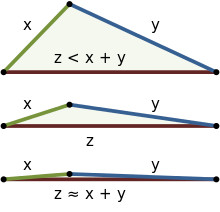
\includegraphics{triangularinequality}
	\end{figure}

We want to show that BFS computes the shortest path $\delta(s,v)$ correctly. We will do it showing first that the distance computed by the BFS procedure bound $\delta(s,v)$ from above.

\begin{theorem}
Suppose we run BFS on a graph $G$ from node $s$ then $v.d \geq \delta(s,v)$. The proof is by induction on the number of \texttt{ENQUEUE} operations. The base case is when only $s$ is in the queue so 
$s.d = 0  = \delta(s,s)$ and $v.d = \infty \geq \delta(s,v)$. Suppose that the hypotesis holds for a number of enqueue operation and in particular that an undiscovered vertex is enqueue from a parent $u$. The inductive hypothesis implies that $u.d \geq \delta(s,u)$. BFS computes the path from $s$ to $v$ composing the path from $s$ to $u$ and adding an edge from $u$ to $v$. this means that: $v.d = u.d +1$
From the theorem \ref{theo:triangular_inequality} follows that $v.d = u.d +1 \geq \delta(s,u) +1 \geq \delta(s,v)$.
\end{theorem}

We have bounded BFS path length from $s$ from above. BFS computes a path which is clearly always less or equal shorter than the shortest possible one. We move on proving that the path it computes are actually the shortest possible so $v.d = \delta(s,v)$.
We now shows that BFS manage in its queue at most two distinct distance values.

\begin{theorem}{\textbf{BFS computes the shortest path from $s$ to all reachable nodes}\hfill \\}
Suppose that for some node (pick up the closest to $s$) $v.d \neq \delta(s,v)$,  then follows that $v.d \geq \delta(s,v)  \wedge \; v.d \neq \delta(s,v) \Rightarrow  v.d > \delta(s,v) $. Let $(u,v)$ an edge then it follows that $\delta(s,v) = \delta(s,u) + 1 = u.d +1$ since $v$ is the first node for which the inequality hold than the BFS path from $s$ to $u$ is the shortest possible\footnote{$\delta(s,u) = u.d$}.
Putting all together we obtain\footnote{$\delta(s,v) = \delta(s,u) + 1 = u.d +1$} 
\[
v.d > u.d + 1 
\]

Consider now the status of $v$ at the time $u$ is explored by BFS procedure. It can be one of the following three cases:
\begin{enumerate}
\item $v$ is UNDISCOVERED: so its distance from $s$ will be $u.d +1 \Rightarrow$ (\textbf{CONTRADICTION)}
\item $v$ was already processed (earlier): $v.d \leq u.d \Rightarrow$ \textbf{(CONTRADITION)}
\item $v$ is DISCOVERED but not PROCESSED: This means that $v$ was discovered when processing a vertex $w$ before $u$ was examined. This also implies that $w$ was processed before $u$ and hence queued before $u$. This implies that $ w.d \leq u.d \Rightarrow w.d+1 \leq u.d +1$. Now, $v$ was discovered by $w$ so its distance from $s$ is $w.d+1$. This allows us to conclude that $v.d \leq u.d+1 \Rightarrow$\textbf{(CONTRADICTION)}.
\end{enumerate}
\end{theorem}

BFS build the so called \textit{Breadth tree} which consist of all the simple (and shortest) paths from $s$ to any reachable (from $s$) vertices \footnote{Those vertices which have a not null parent}. Note that this tree is not unique, and depends on the order in which nodes in the adjacency lists are examined. Node can be discovered using different edges.


\subsection{Exercices}
%---Problem------------
\begin{problem}
There are two types of professional wrestlers:  babyfaces  ( good guys) and
heels ( bad guys ). Between any pair of professional wrestlers, there may or
may not be a rivalry. Suppose we have n professional wrestlers and we have a list
of r pairs of wrestlers for which there are rivalries. Give an O.n C r/-time algo-
rithm that determines whether it is possible to designate some of the wrestlers as
babyfaces and the remainder as heels such that each rivalry is between a babyface
and a heel. If it is possible to perform such a designation, your algorithm should
produce it.
\begin{solution}
This is a two-color graph coloring problem which is easily solvable in linear time (we are also asking if the graph is bipartite).
We create a node for each professional wrestler and connect them using the relation coded into the $r$ pairs. We then start coloring the graph from a random node and at each level we switch color. If we encounter a node which was previously colored with a different color\footnote{This means that two vertex on a edge that were preivously coloured with different colors are now of the same color.} the such graph is not bipartite and so is not possible to divide \textit{babyfaces} from \textit{heels}. If we consume all the nodes, then the output graph is a proper bipartition.
\end{solution}


\end{problem}



%---Problem------------
\begin{problem}
\textit{Show the d and $\pi$ values that result from running breadth-first search on graph pictured in figure \ref{fig:graphex}, using vertex 3 as the source}.


	\begin{figure}
	\label{fig:graphex}
	\centering
		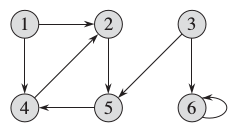
\includegraphics{graphEx}
	\end{figure}
\begin{solution}
\[d(3) = 0 , d(1) = \infty , d(5) = d(6) = 1 , d(4) = 2 ,d(2) = 3\].
\[d(3) = NIL , \pi(1) = NIL , \pi(5) = \pi(6) = 3 , \pi(4) = 5 ,\pi(2) = 4\].
	\end{solution}
\end{problem}


%---Problem------------
\begin{problem}
\textit{Show the d and $\pi$ values that result from running breadth-first search on graph pictured in figure \ref{fig:graphex2}, using vertex 3 as the source}.


	\begin{figure}
	\label{fig:graphex2}
	\centering
		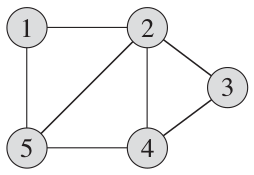
\includegraphics{graphEx2}
	\end{figure}
\begin{solution}
\[d(3) = 0 , d(1) = \infty , d(5) = d(6) = 1 , d(4) = 2 ,d(2) = 3\].
\[d(3) = NIL , \pi(1) = NIL , \pi(5) = \pi(6) = 3 , \pi(4) = 5 ,\pi(2) = 4\].
	\end{solution}
\end{problem}



\subsection{Depth-first}
Depth-first search explores edges out of the most recently discovered vertex $v$ that still has unexplored edges leaving it.
Once all of $v$'s edges have been explored, the search \textit{backtracks} to explore edges
leaving the vertex from which $v$ was discovered. This process continues until we
have discovered all the vertices that are reachable from the original source vertex.
As for breadth-first if any undiscovered vertices remain, then depth-first search selects one of them as
a new source, and it repeats the search from that source until all the vertices are discovered.
As in breadth-first search, depth-first search colors vertices during the search to
indicate their state. Each vertex is initially white, is grayed when it is discovered
in the search, and is blackened when it is finished, that is, when its adjacency list
has been examined completely.
Depth-first also timestamps each node at the time of discovery and when it finishes to process it (consumes its entire adjacency list) in, respectively $v.d$ and $v.f$ s,t, $v.d < v.f$.

\begin{algorithm}
 \KwData{Graph  $G = (V,E)$}
  \For{$v  \in V$}{
	$status[v] = UNDISCOVERED$\;
	$parent[v] = NIL$\;  
  }
 \For{$v  \in V$}{
 	 \If{status[v] == UNDISCOVERED}{
		%visit component that starts in n 	 	
 	 		$DFS-helper(G,v)$\;
  }
 }
\caption{DFS procedure}
\end{algorithm}


\begin{algorithm}
 \KwData{Graph  $G = (V,E)$, start node $s$}

$time = time +1$\;
$s.d = time$ \tcp*{discovery time for $s$}
 \For{$v  \in ADJ[V]$}{
 	 \If{status[v] == UNDISCOVERED}{
		%visit component that starts in n 	 	
			$parent[v] = s$\;
 	 		$DFS-helper(G,v)$\;
 	 		
  }
 }
 $status[s] = PROCESSED$\;
 $time = time +1$\;
 $s.f = time$\;
\caption{DFS-helper procedure. Start the DFS from a node $s$}
\end{algorithm}

Every time in the main procedure DFS-helper is called, $v$ becames a root of a depth visit tree.
Note that the resulting visiting forest  is not unique and may depend in the order in which the vertices are processed. This is not usually a problem in practice since we can equivalently use any of the possible ouput forest.

What is the running time of DFS? The main procedure loops over all the vertices and call DFS-helper.
DFS-helper is executed only once per vertex (only when their status is undiscovered) and have it loops over all the edges in $ADJ[v]$. The sum of all edges is clearly $|E|$, hence the overall complexity is $\Theta
(V+E)$

\subsubsection{Analysis and properties of DFS}
DFS yelds to imponrtant and valuable information about the structure of the graph. The prodecessor subgraph $G_{\pi} = (V,E_{\pi})$ subgraph is a forest of trees and reflect the recursive structure of the calls to DFS-helper.
Another important property is that dicovery and finish time have the so called parenthesis structure, in the sense that the history of discovery and finish time of the vertices make up a well formed nested expression of parenthesis.

\begin{theorem}{\textbf{Parenthesis theorem for DFS}}
In any DFS visit for any pair of vertices $u$ and $v$ one and only one of the following property holds (see image \ref{fig:parenthesisproperty}).
Note that $\forall \; v \in V \; v.d < v.f$
\begin{enumerate}
\item The intervals $(v.d,v.f)$ and  $(u.d,u.f)$ are completly disjoint i.e. $v.f < u.d$ or $u.f < v.d$. It means that neither $v$ or $v$ are descendant of the other in the DFS forest. They are discovered in different recursive branches of the DFS-helper procedure.
\item The $u$'s interval is completly overlaps with $v$'s i.e.  $v.d < u.d$ and $v.f > u.f$. It means that $u$ is direct descendent of $v$.
\item The $v$'s interval is completly overlaps with $u$'s i.e. $u.d < v.d$ and $u.f > v.d$ . It means that $v$ is direct descendent of $u$.
\end{enumerate}

\end{theorem}

	\begin{figure}[h]
	\centering
	\label{fig:parenthesisproperty}
		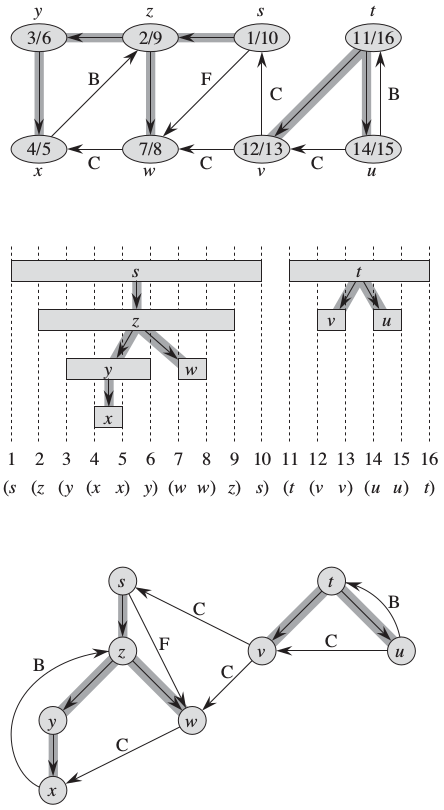
\includegraphics[scale=0.8]{parenthesisproperty}
	\end{figure}



\subsection{Topological Sort}
Topological sort is an operation on directed acyclic graphs (also called DAGs). It orders vertices such that all directed edges goes from left to right or right to left (depending on the choosen ordering). Such ordering exists only on direct graphs (because each undirected edge is a cycle of length 2) and on acyclic graphs (because in a cycle there is no way to go in a specified direction withouth going back to the starting point, hence for two nodes $i,j$ both $i$ after $j$ and $ j$ after $i$ hold). 
Each DAG has at least one topological sort. DAG are the natural representation of a number of important problems, such job scheduling for instance where each job is a vertex and edges represent dependencies between them (and edge $(i,j)$ means that job $i$  need to be performed before job $j$).
Topological sortin can be performed using DFS and in particular a graphs ia a DFs if and only if no back edges are encountered during the visit.

In particular when examining an edge $(x,y)$ from $x$, $y$ can be in one of the following states:
\begin{description}
\item [undiscovered]: $y$ appers then after $x$ in the topological sort
\item [discovered but no processed]: it means that it is a back edge (a cycle exists in the graph). The graph is not a DAG, so no topological sort exists for it.
\item [processed]: $y$ was discovered and processed before $x$, so it appears before in the topological sort
\end{description}



%---Problem------------
\begin{problem}\textit{{Prove by induction that exists only one path between each vertices of a tree}}

\begin{solution}
We will use induction on the level tree level. We can think about two distinc base cases at least. Tree of height 1 and 2. Tree with height 1 have only one node so the property holds trivially. Node with height 2 have one $N_c+1$ nodes where $N_c$ is the number of child of the root $r$. Each child is connected to the root by a unique edge so there exists a unique path between any child and the root. Children are not connected each other so any path is forced to contain $r$. So the only legal path between childre $i$ and $j$ , $i \neq j$ is of the following form $i \rightarrow p \rightarrow j$.

Suppose now that this property holds for tree with height up to $n$ and see if the property holds for trees with height $n+1$.The nodes at level $n+1$ does not add any edges at levels $n' < n+1$ so this does not add any path between any nodes at upper levels. We will shows that exists a unique path between any node at level $n'$ and $n+1$ and between leafs in two distinc steps.
\begin{itemize}
\item The path between the leaf $i$ with parent $p(i)$and a non leaf $o$ is forced to contain the unique edge connecting $i$ and $p(i)$. Since there exists a unique path between $o$ and $p(i)$ there is only one way to construct a path between $o$ and $i$ and is the following: $o \rightarrow p(i) \rightarrow i$
\item The path between two leafs $i,j$ with parents $p(i),p(j)$ respectively is forces to contains edges $(i,p(i)),(j,p(j))$ since those are the only edges connecting the them to the upper levels. Let $c$ the first common ancestor of $i,j$ which is clearly at level $n'<n+1$. There is unique path between $c$ and both $p(i)$ and $p(j)$ so the only possible path is the following: $i \rightarrow p(i) \rightarrow c \rightarrow p(j) \rightarrow j$.
\end{itemize}
\end{solution}


\end{problem}


%---Problem------------
\begin{problem}{\textit{Prove that in BFS every edges is either a tree edge or a cross edge. Shows that in cross edges $(x,y)$ x is neither an ancestor nor a descendant of y (not immediate).}}

\begin{solution}
Let's begin saying that edge $(x,y) $ is classified as tree or cross depending on the status the endpoint $y$ and that we first examine all edges going out from $x$ before examining another node. All nodes from level $l$ are fully examined before moving to nodes at deeper levels.
If $y$ is in an undiscovered status it means that no other node $z \neq x \neq y$ have been examined such that an edge $(z,y)$ exists so far. It it then labeled as tree edge (there is no other node at previous level which connects to $y$).
Suppose that $y$ has status \textit{discovered}. This means that there exists already an edge with endpoint $y$ in the BFS tree and the edge is labeled as cross. Each node can be only in one of those two state hence each edge is labeled either as cross or tree.In other words another node from the same level has discovered $y$ first. 
In a cross edge $(x,y)$ $x$ cannot be a non immediate ancestor of $y$ because if it was the case we would have used that edge as tree edge when visiting $x$.
The same hold for an non immediate descendant because the graph is undirected and we would have visited $y$ before $x$ and used $(y,x)$ as tree edge.

Notice that BFS consider edges from level $l$ to level $l+1$. Being a non immediate ancestor or descendant of a node implies to be processed at previous levels.


\end{solution}

\end{problem}

%---Problem------------
\begin{problem}{\textit{Give a linear algorithm to compute the chromatic number of graphs where each vertex has degree at most 2. Must such graph be dipartite?}}\footnote{The chromatic number of a graph G is the smallest number of colors needed to color the vertices of G so that no two adjacent vertices share the same color (Skiena 1990, p. 210), i.e., the smallest value of k possible to obtain a k-coloring. Minimal colorings and chromatic numbers for a sample of graphs are illustrated above}

\begin{solution}
We first derive un upper bound for the chromatic number, i.e. which is the minimum number $U_\gamma(G)$ for a graph $G$  s.t. $\gamma(G) \geq U_\gamma(G)$. Let's first say that each connected component has a chromatic number which is independent from the others and the graph chromatic number would be the maximum between all the component's chromatic numbers.
Graphs of this kind are very similar to cycle graphs in which each connected component have at most only two nodes with degree one. 
Cycle graph have chromatic number 2 or tree depending on the number of vertices (2 if even, 3 if odd).
When a connected component has two nodes with degree one, then its chromatic number is always 2 (is like a list in which head and tail have degree 1). 
A simple algorithm that work in linear time and constant space is the folloowing. If the number of nodes is even return two. Otherwise use DFS from a node $s$ coloured in white. Each time a node is discovered we color it with the opposite color of its parent. Each time we color a vertex we check for any conflict in color. If we find a conflict we simply pick up a new color to be used for the current vertex.
Note that there will be only one place for conflict so no more than one node will need a "spare" color.

Note that there is a theorem that generalize this result. The Brooks's theorem which state that for any graph with degree at most $\Delta$ its chromatic number is $\Delta$. Two exception to this rule are the complete and cycle graph with an odd number of vertices (infact in this exercice for cycle graph we require 3 colors).



\end{solution}

\end{problem}


%---Problem------------
\begin{problem}{\textit{In breadth-first and depth-first search, an undiscovered node is marked discov-
ered when it is first encountered, and marked processed when it has been completely searched. At any given moment, several nodes might be simultaneously in the discovered state.}}

\textit{\begin{itemize}
\item Describe a graph on $n$ vertices and a particular starting vertex $v$ such that
$\Theta(n)$ nodes are simultaneously in the discovered state during a breadth-first search
starting from $v$.
\item Describe a graph on $n$ vertices and a particular starting vertex $v$ such that $\Theta(n)$
nodes are simultaneously in the discovered state during a depth-first search starting
from $v$
\item Describe a graph on $n$ vertices and a particular starting vertex $v$ such that at
some point $\Theta(n)$ nodes remain undiscovered, while $\Theta(n)$ nodes have been processed
during a depth-first search starting from $v$. (Note, there may also be discovered nodes.)
\end{itemize}}

\begin{solution}
\begin{itemize}
\item The Star Graph (see figure \ref{fig:star} ) $S_k$ using as starting node the central one (the unique with degree $k-1$), or the complete graph $K_k$ (see figure \ref{fig:complete}) using any node as starting point.
	\begin{figure}
		\centering
		\label{fig:star}
		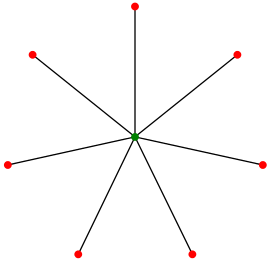
\includegraphics[width=3cm]{start.png}
		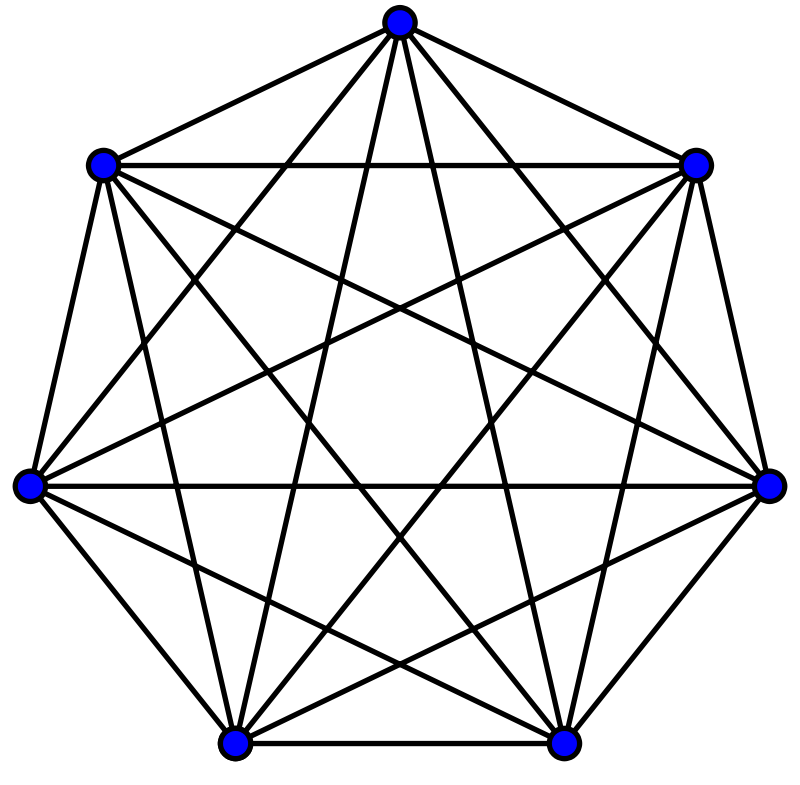
\includegraphics[width=3cm]{complete.png}
		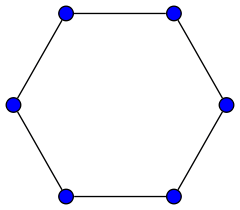
\includegraphics[width=3cm]{cycle.png}
		\caption{Star complete and a cycle graph examples.}
	\end{figure}
\item The cycle graph $C_k$ (see figure \ref{fig:cycle}) using any node as starting point.
	
\item A graph with $n$ nodes s.t. two half of the nodes are organized as a list of nodes $\frac{n}{2}$, and each their heads share a node (which is used as starting point). DFS will eventually process one branch leaving the other one undiscovered. Since each branch has $\frac{n}{2} = \Theta(n)$ nodes the constraints are satisfied.
\end{itemize}




\end{solution}
\end{problem}

%-----END OF CHAPTER GRAPH---------------------------

\chapter{Set}
\section{MultiSet}

\chapter{Associative Array - Dictionary}
\section{Map}
\section{MultiMap}
\section{Hash table - Hash Map}
\iffalse
http://www.tommyds.it/doc/benchmark.html
\fi